%================================================================
\section{Results and Discussion}\label{sec:Results}
%================================================================

%===============================================================
\subsection{Heat Equation}\label{sec:heateq results}
%===============================================================
Accompanying notebook: \href{https://github.com/nicolossus/FYS-STK4155-Project3/blob/master/notebooks/heat_pde_with_fe_and_tf.ipynb}{heat\_pde\_with\_fe\_and\_tf.ipynb}.

%===============================================================
\subsubsection{Forward Euler}
%===============================================================
Nx = 11
Nt = 199

Max diff: 0.04009472326320718
Mean diff: 0.003186288853514369

\autoref{fig:heat_fe}
\begin{figure}[H]
\centering
\subfloat[]{{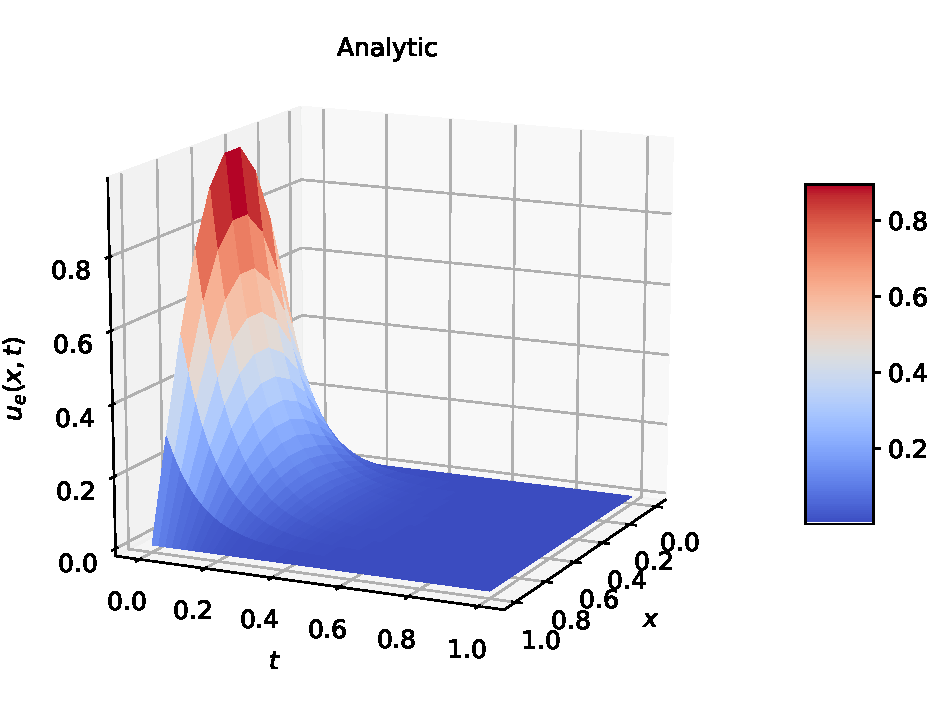
\includegraphics[scale=0.48]{latex/figures/heat_ana_fe.pdf}}}
\qquad
\subfloat[]{{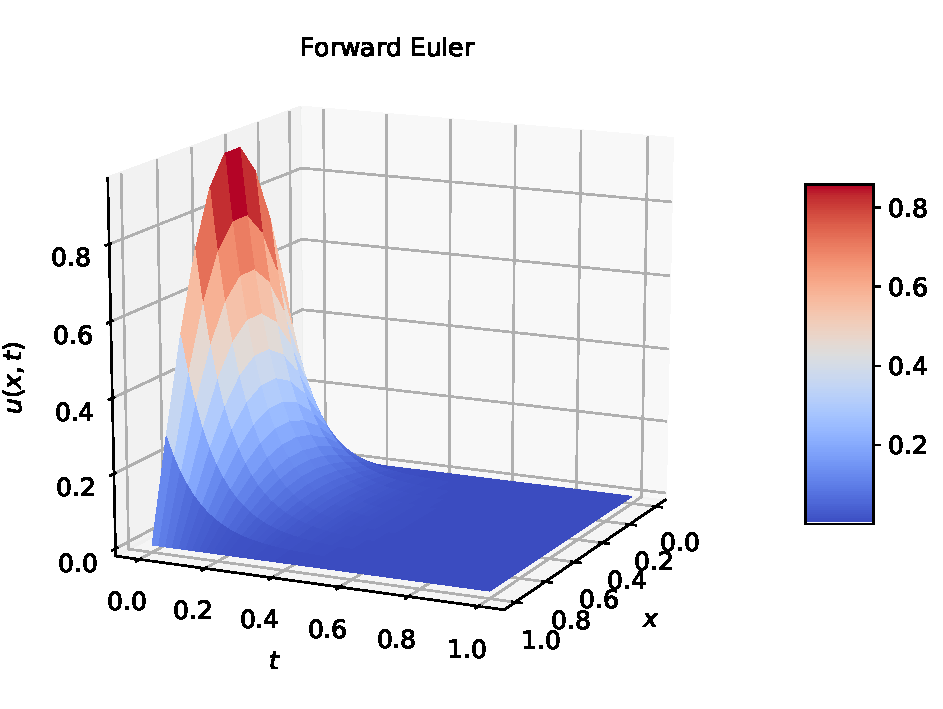
\includegraphics[scale=0.48]{latex/figures/heat_fe.pdf}}}
\qquad
\subfloat[]{{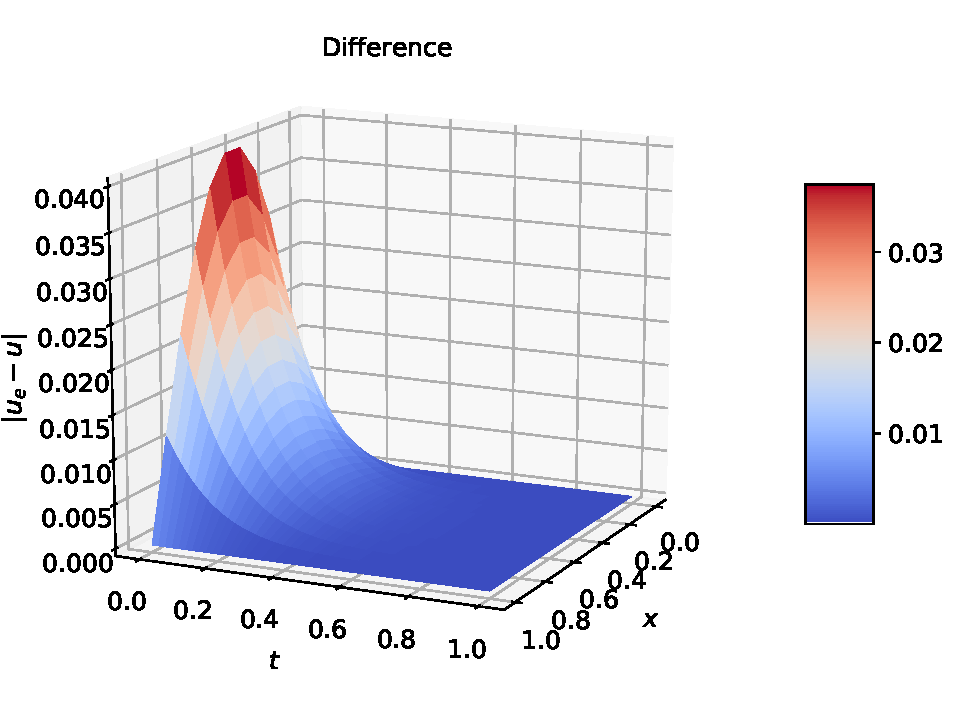
\includegraphics[scale=0.5]{latex/figures/heat_diff_fe.pdf}}}
\caption{FE heat}
\label{fig:heat_fe}
\end{figure}

CPU benchmark
Number of iterations: 1000
FE mean CPU time: 0.00158 secs

Simulations with the Forward Euler scheme show that the time step restriction, $F \leq 1/2$, which means $\Delta t \leq \Delta x^2 / (2\alpha)$, may be relevant in the beginning of the diffusion process, when the solution changes quite fast, but as time increases, the process slows down, and a small $\Delta t$ may be inconvenient.

%===============================================================
\subsubsection{FFNN Model 1}
%===============================================================

Model 1: Train on spatial and temporal points as dictated by FE stability criterion

Nx = 11
Nt = 199
2 layers + output, [150, 50, 1], [tanh, sigmoid, none] 
1000 epochs
Adam, initial lr=0.01
Step: 1000, Loss: 0.008064055285575904
Training FFNN CPU time: 147.62562 secs

\autoref{fig:heat_nn1} Plot solution on the grid FFNN is trained on

Max diff: 0.008466789818225778
Mean diff: 0.0029635112954797672

\begin{figure}[H]
\centering
\subfloat[]{{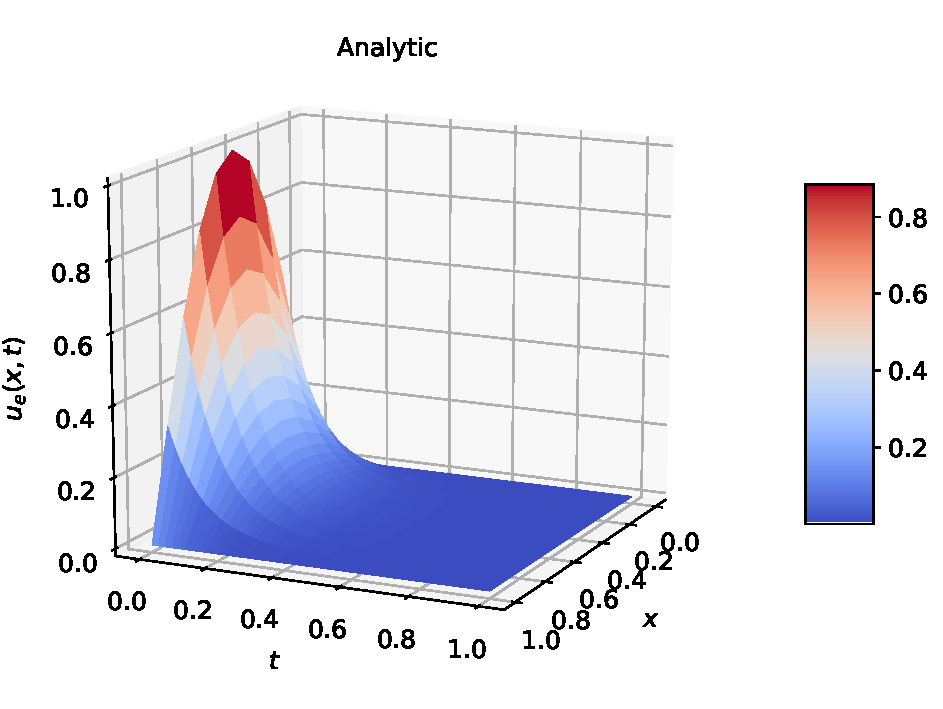
\includegraphics[scale=0.48]{latex/figures/heat_ana_nn1.pdf}}}
\qquad
\subfloat[]{{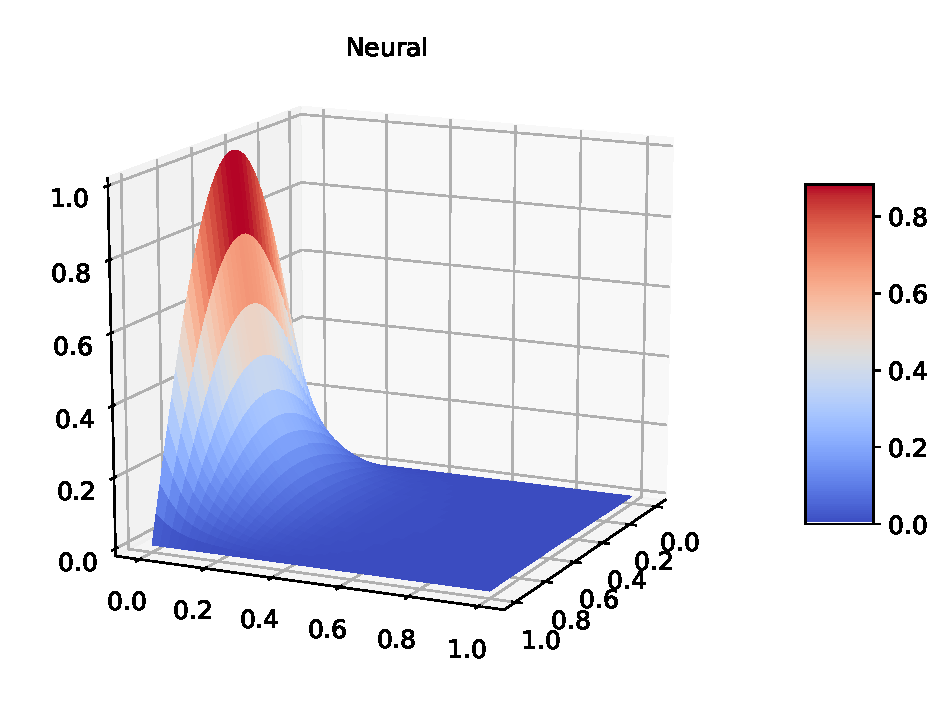
\includegraphics[scale=0.48]{latex/figures/heat_nn1.pdf}}}
\qquad
\subfloat[]{{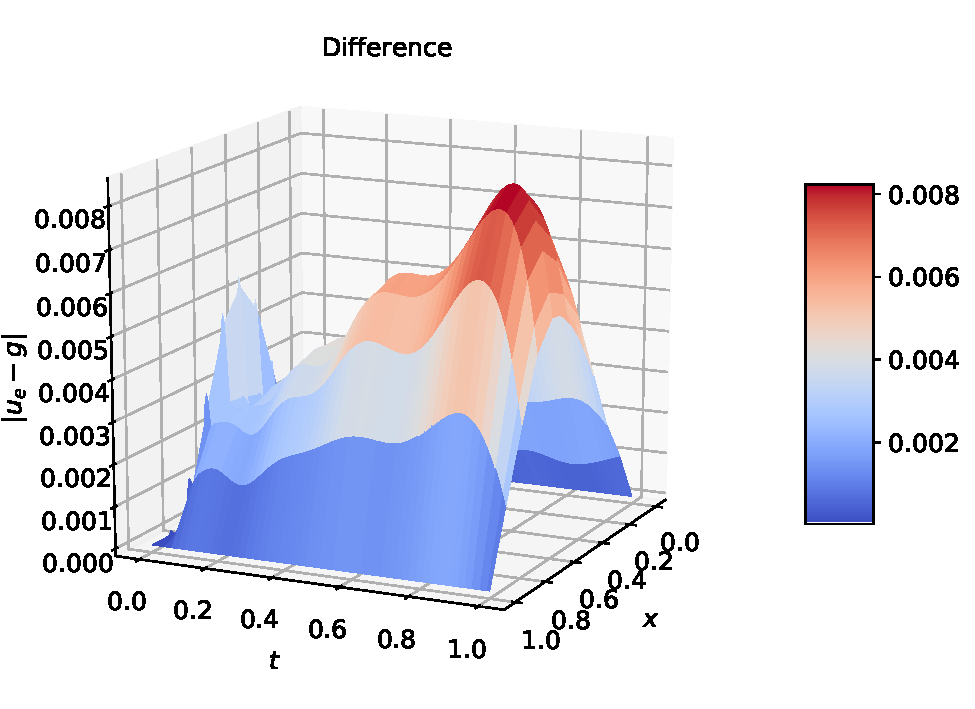
\includegraphics[scale=0.5]{latex/figures/heat_diff_nn1.pdf}}}
\caption{Model 1, Plot solution on the grid FFNN is trained on}
\label{fig:heat_nn1}
\end{figure}

\autoref{fig:heat_nn2} Plot solution on a larger grid than FFNN is trained on, i.e., points must be interpolated

301, 301 points

Max diff: 0.008467176325477247
Mean diff: 0.0032787069037113277

\begin{figure}[H]
\centering
\subfloat[]{{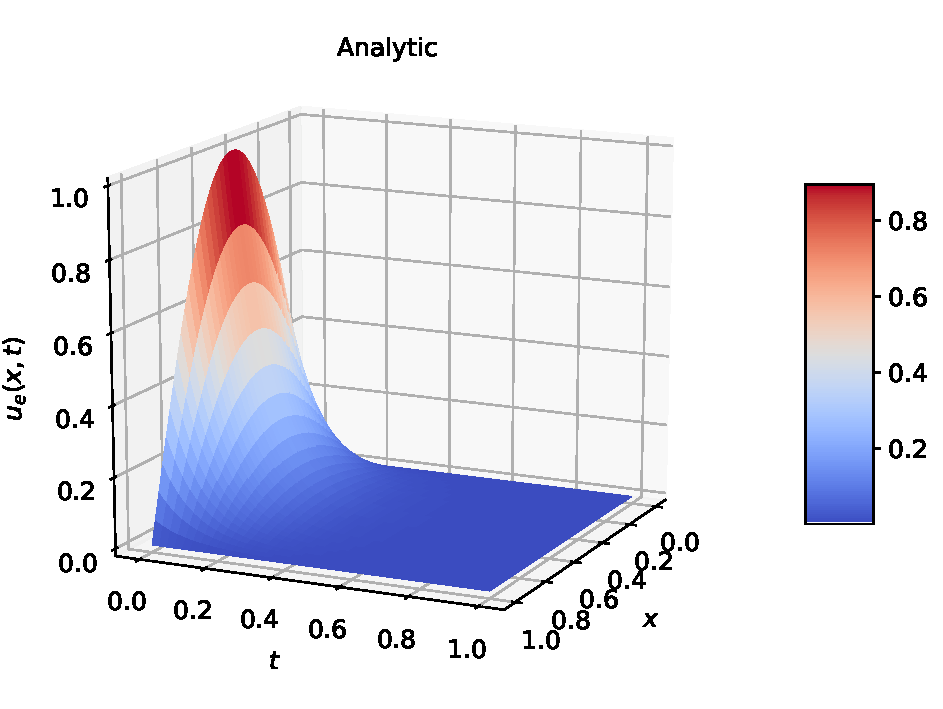
\includegraphics[scale=0.48]{latex/figures/heat_ana_nn2.pdf}}}
\qquad
\subfloat[]{{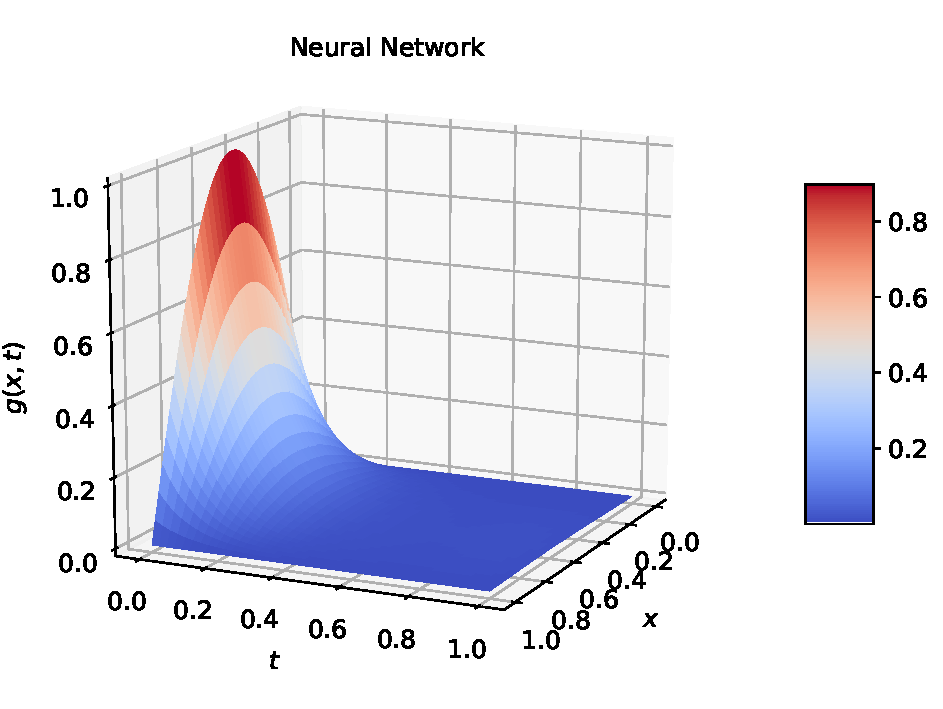
\includegraphics[scale=0.48]{latex/figures/heat_nn2.pdf}}}
\qquad
\subfloat[]{{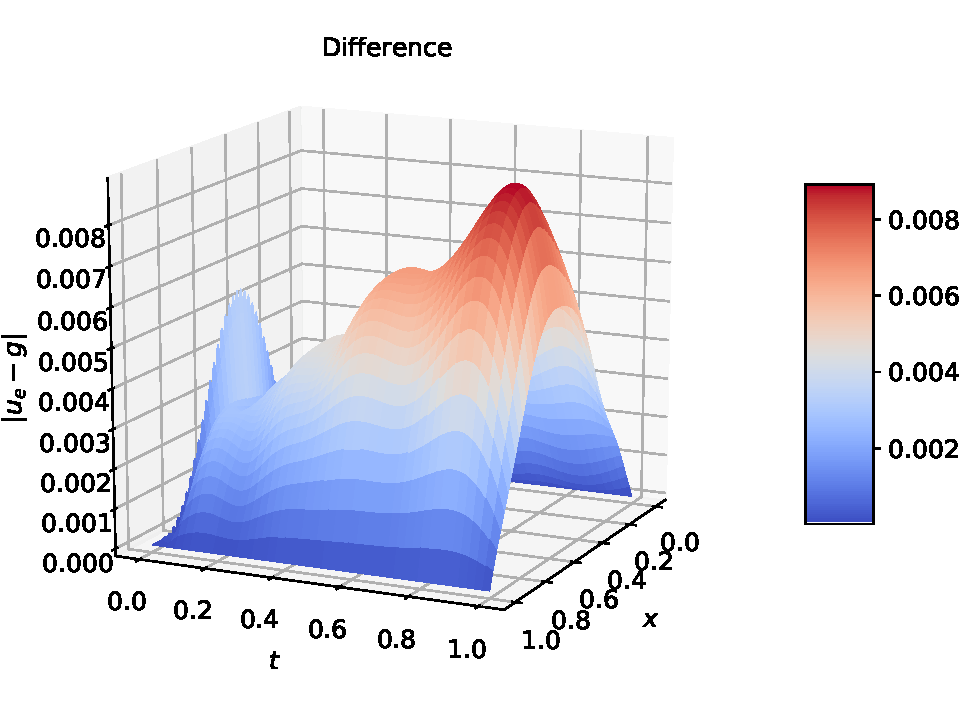
\includegraphics[scale=0.5]{latex/figures/heat_diff_nn2.pdf}}}
\caption{Model 1, Plot solution on a larger grid than FFNN is trained on, i.e., points must be interpolated}
\label{fig:heat_nn2}
\end{figure}

%===============================================================
\subsubsection{FFNN Model 2}
%===============================================================
Model 2: Train on equal number of spatial and temporal points

Nx = 11
Nt = 11
2 layers + output, [150, 50, 1], [tanh, sigmoid, none] 
1000 epochs
Adam, initial lr=0.01
Step: 1000, Loss: 0.008064055285575904
Training FFNN CPU time: 147.62562 secs
Step: 1000, Loss: 0.0027709536906761877
Training FFNN CPU time: 42.11612 secs

\autoref{fig:heat_nn3} Plot solution on the grid FFNN is trained on

Max diff: 0.026960711104318635
Mean diff: 0.0029851059330631173

\begin{figure}[H]
\centering
\subfloat[]{{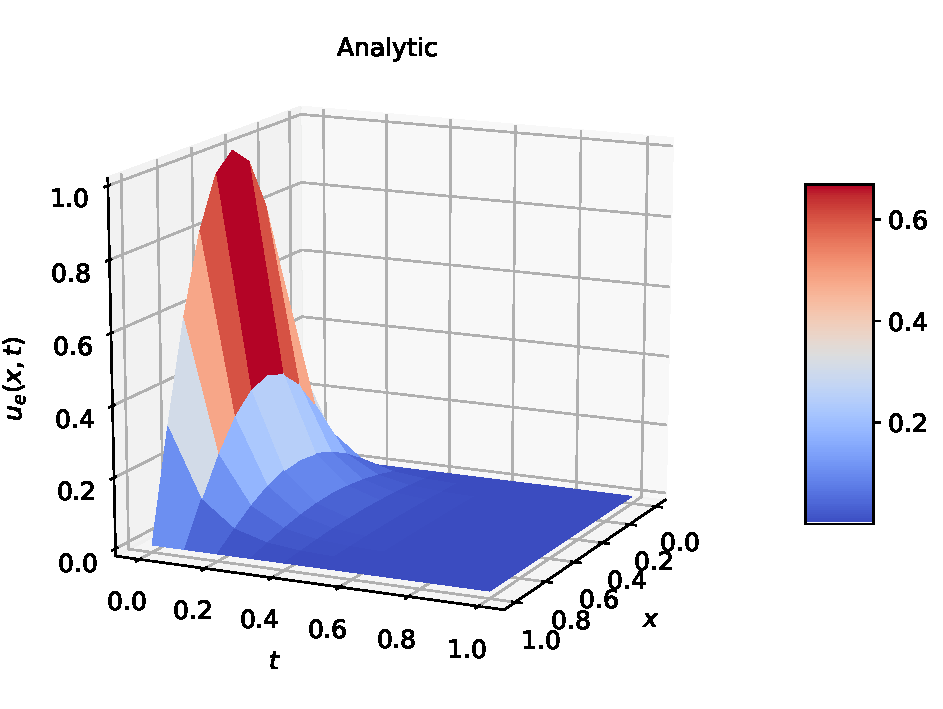
\includegraphics[scale=0.48]{latex/figures/heat_ana_nn3.pdf}}}
\qquad
\subfloat[]{{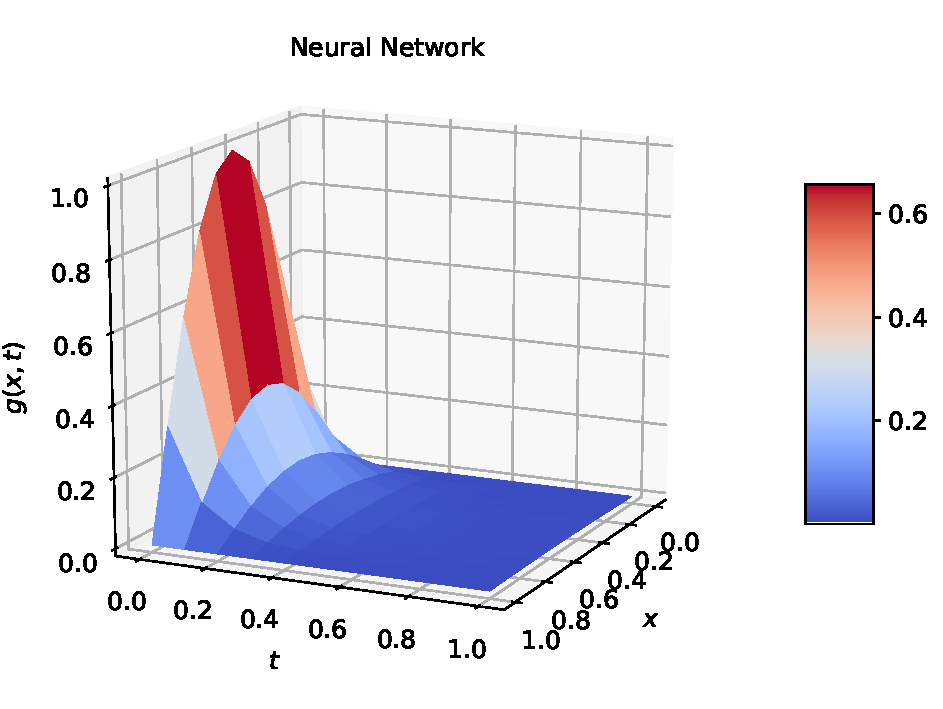
\includegraphics[scale=0.48]{latex/figures/heat_nn3.pdf}}}
\qquad
\subfloat[]{{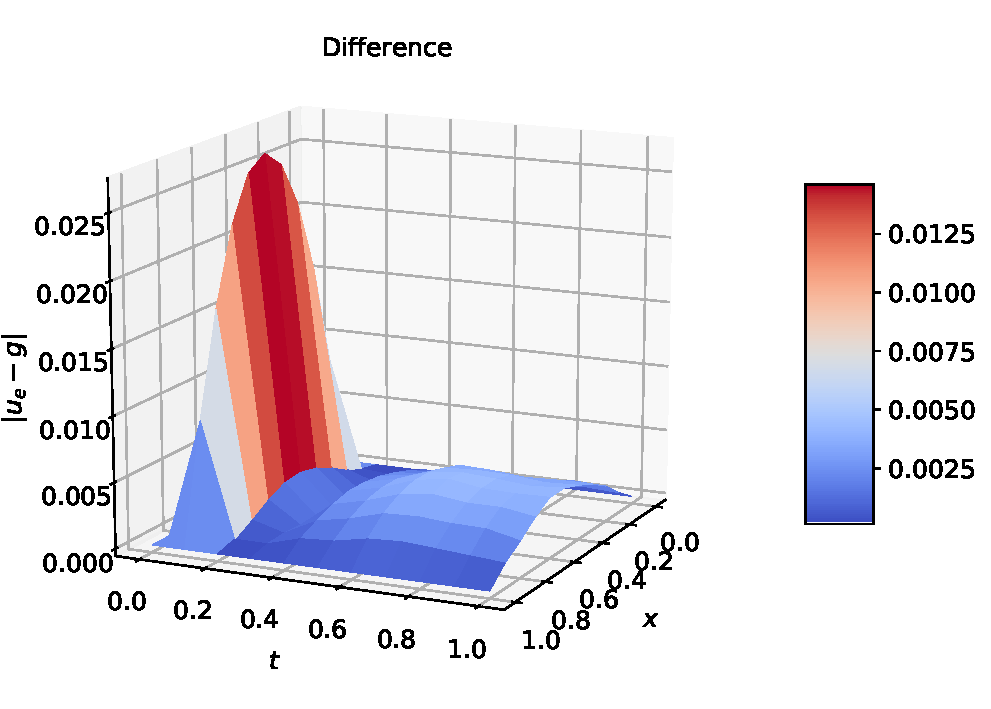
\includegraphics[scale=0.5]{latex/figures/heat_diff_nn3.pdf}}}
\caption{Model 2, Plot solution on the grid FFNN is trained on}
\label{fig:heat_nn3}
\end{figure}

\autoref{fig:heat_nn4} Plot solution on a larger grid than FFNN is trained on, i.e., points must be interpolated

301, 301 points

Max diff: 0.03215260678986426
Mean diff: 0.003950743671390742

\begin{figure}[H]
\centering
\subfloat[]{{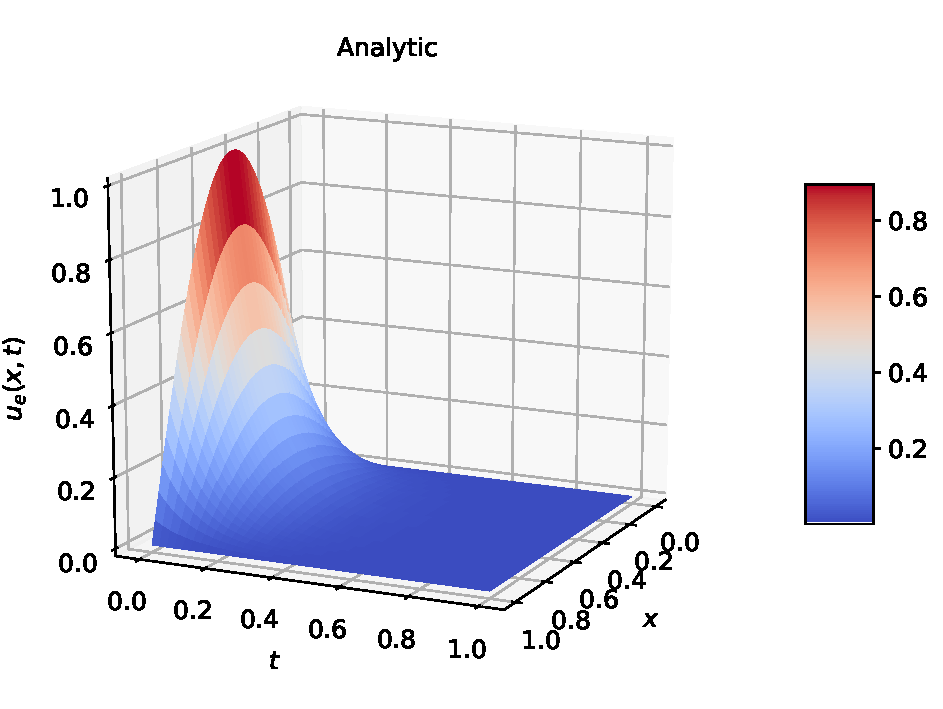
\includegraphics[scale=0.48]{latex/figures/heat_ana_nn4.pdf}}}
\qquad
\subfloat[]{{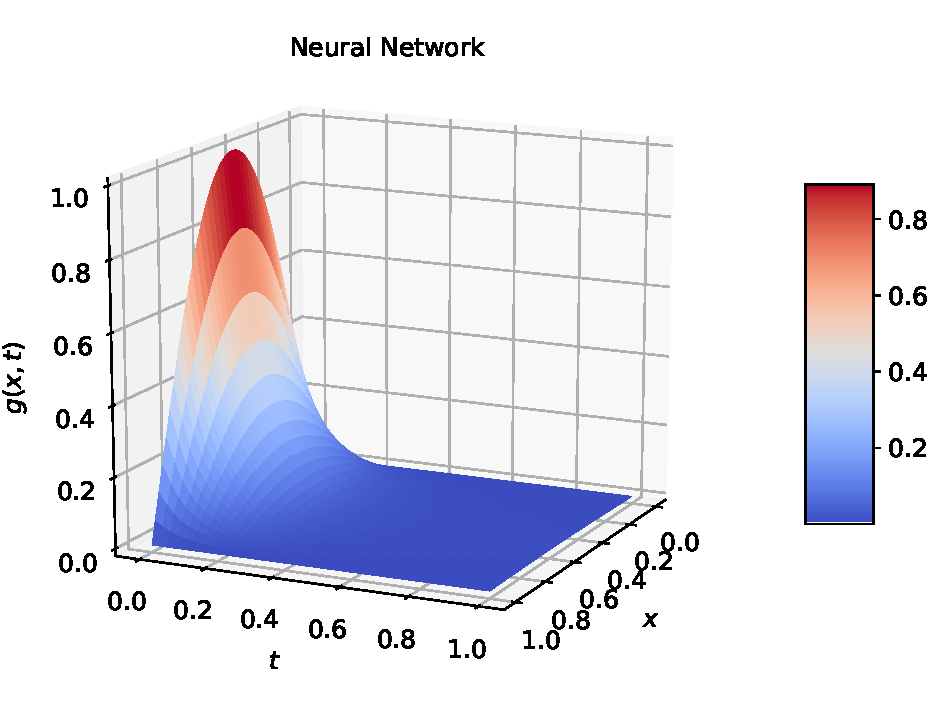
\includegraphics[scale=0.48]{latex/figures/heat_nn4.pdf}}}
\qquad
\subfloat[]{{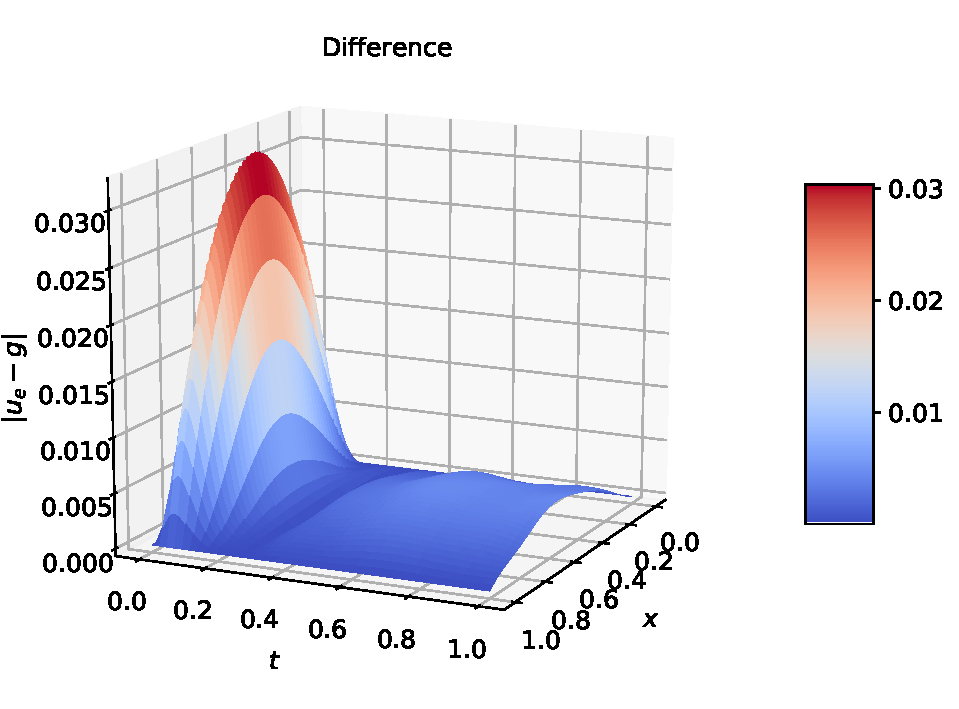
\includegraphics[scale=0.5]{latex/figures/heat_diff_nn4.pdf}}}
\caption{Model 2, Plot solution on a larger grid than FFNN is trained on, i.e., points must be interpolated}
\label{fig:heat_nn4}
\end{figure}

%===============================================================
\subsubsection{Home-made FFNN}
%===============================================================


%===============================================================
%===============================================================
\subsection{Eigenvalue Problem}\label{sec:eigenvalue results}
%===============================================================
%===============================================================

Accompanying notebook: \href{https://github.com/nicolossus/FYS-STK4155-Project3/blob/master/notebooks/eigenvalue_tf.ipynb}{eigenvalue\_tf.ipynb}.

%===============================================================
\subsubsection{Benchmark Problem 1}
%===============================================================

\autoref{tab:parabench1} tabulates the problem and model parameters for Benchmark Problem 1 described in \autoref{sec:benchmark problem 1}. 

\begin{table}[H]
\caption{Problem and model parameters for Benchmark Problem 1.}
\centering
\rowcolors{2}{gray!20}{white}
\begin{tabular}{c|c}
\hline
\hline 
Parameter & Numerical Value
\\
\hline 
\hline 
Initial vector & $\bm{x_0}=(1,0,0)$
\\
Simulation time & 1
\\
Number of time points (Euler) & 101
\\
Number of time points (FFNN) & 11
\\
Number of epochs (FFNN) & 2000
\\
\hline
\hline 
\end{tabular}
\label{tab:parabench1}
\end{table}


\autoref{fig:benchrun1} shows the results for Benchmark Problem 1. The computed Rayleigh quotients and the absolute error relative to the eigenvalue computed by Numpy are tabulated in \autoref{tab:eigbench1}. 

\begin{figure}[H]
\centering
\subfloat[]{{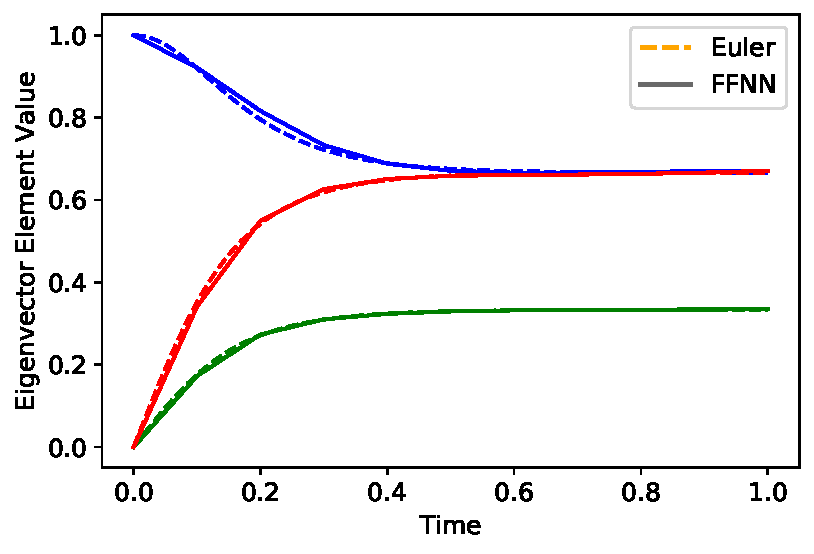
\includegraphics[scale=0.6]{latex/figures/eigvec_comp_benchrun1.pdf}}}
\qquad
\subfloat[]{{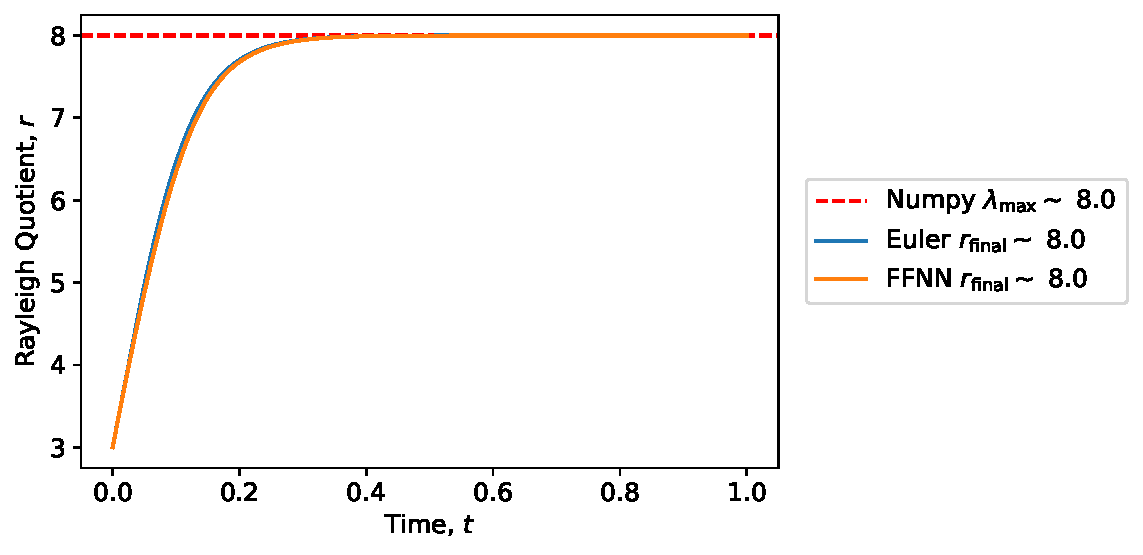
\includegraphics[scale=0.6]{latex/figures/eigval_benchrun1.pdf}}}
\caption{Results for Benchmark Problem 1 with a $3\times 3$ real symmetric matrix, $A$. \textbf{(a)} shows the components of the computed steady-state vector as a function of time. The dashed lines are the components computed by Euler's method and the solid lines are computed by the FFNN model. The dotted lines are the normalized (unit "length") eigenvector components corresponding to the largest eigenvalue computed directly from the matrix by Numpy's linalg.eig. \textbf{(b)} shows the computed Rayleigh quotients, $r$, as a function of time for both Euler's method and the FFNN model and the largest eigenvalue, $\lambda_\mathrm{max}$, of the matrix computed by Numpy's linalg.eig as well. The final Rayleigh quotients are rounded to 5 decimal points.}
\label{fig:benchrun1}
\end{figure}

\begin{table}[H]
\caption{The computed Rayleigh quotients at the final simulation time for both Euler's method and the FFNN model. The absolute error relative to the eigenvalue computed by Numpy is also listed.}
\centering
\rowcolors{2}{gray!20}{white}
\begin{tabular}{c|c|c}
\hline
\hline 
Method & Rayleigh Quotient & Absolute Error
\\
\hline 
\hline 
Numpy & 8.0 & –
\\
Euler & 7.99999993 & $6.007 \cdot 10^{-8}$  
\\
FFNN & 7.99999803 & $1.967 \cdot 10^{-6}$
\\
\hline
\hline 
\end{tabular}
\label{tab:eigbench1}
\end{table}

The eigenvalue computed by Numpy correspond to the analytical solution in this case. Euler achieves higher accuracy

DISCUSSION

%===============================================================
\subsubsection{Benchmark Problem 2}
%===============================================================

The problem and model parameters for Benchmark Problem 2, described in \autoref{sec:benchmark problem 2}, are the same as for Benchmark Problem 1 tabulated in \autoref{tab:parabench1}. The difference for this problem is that the matrix has opposite signs, $-A$, i.e. we are finding the smallest eigenvalue of $A$.

\autoref{fig:benchrun2} shows the results for Benchmark Problem 2. The computed Rayleigh quotients and the absolute error relative to the eigenvalue computed by Numpy are tabulated in \autoref{tab:eigbench2}. 

\begin{figure}[H]
\centering
\subfloat[]{{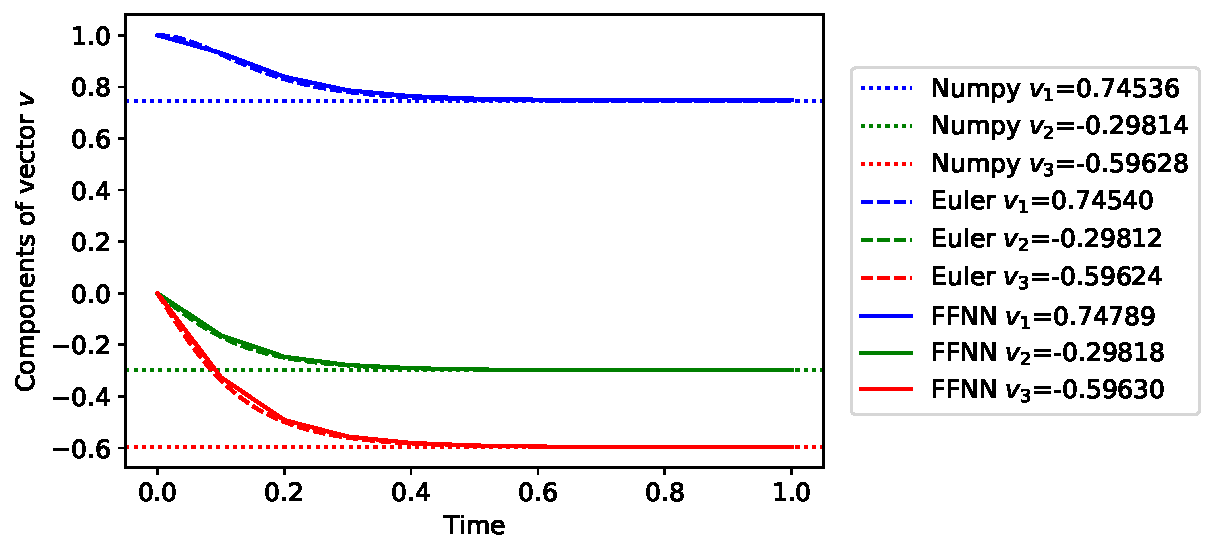
\includegraphics[scale=0.6]{latex/figures/eigvec_comp_benchrun2.pdf}}}
\qquad
\subfloat[]{{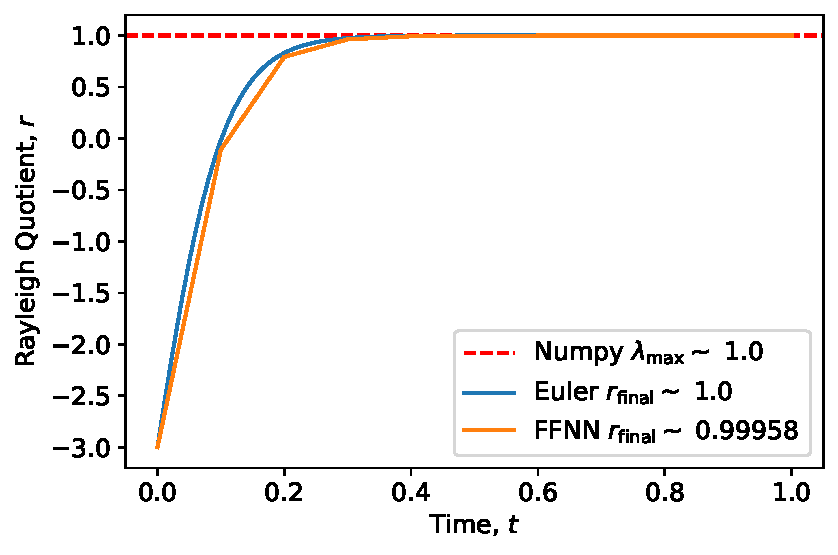
\includegraphics[scale=0.6]{latex/figures/eigval_benchrun2.pdf}}}
\caption{Results for Benchmark Problem 2 with a $3\times 3$ real symmetric matrix, $-A$. \textbf{(a)} shows the components of the computed steady-state vector as a function of time. The dashed lines are the components computed by Euler's method and the solid lines are computed by the FFNN model. The dotted lines are the normalized (unit "length") eigenvector components corresponding to the largest eigenvalue computed directly from the matrix by Numpy's linalg.eig. \textbf{(b)} shows the computed Rayleigh quotients, $r$, as a function of time for both Euler's method and the FFNN model and the largest eigenvalue, $\lambda_\mathrm{max}$, of the matrix computed by Numpy's linalg.eig as well. The final Rayleigh quotients are rounded to 5 decimal points.}
\label{fig:benchrun2}
\end{figure}

\begin{table}[H]
\caption{The computed Rayleigh quotients at the final simulation time for both Euler's method and the FFNN model. The absolute error relative to the eigenvalue computed by Numpy is also listed.}
\centering
\rowcolors{2}{gray!20}{white}
\begin{tabular}{c|c|c}
\hline
\hline 
Method & Rayleigh Quotient & Absolute Error
\\
\hline 
\hline 
Numpy & 1.0 & –
\\
Euler & 0.99999995 & $4.112 \cdot 10^{-8}$  
\\
FFNN & 0.99997506 & $2.493 \cdot 10^{-5}$
\\
\hline
\hline 
\end{tabular}
\label{tab:eigbench2}
\end{table}


DISCUSS


%===============================================================
\subsubsection{Benchmark Problem 3}
%===============================================================

\autoref{tab:parabench3} tabulates the problem and model parameters for Benchmark Problem 3 described in \autoref{sec:benchmark problem 3}. 

\begin{table}[H]
\caption{Problem and model parameters for Benchmark Problem 3.}
\centering
\rowcolors{2}{gray!20}{white}
\begin{tabular}{c|c}
\hline
\hline 
Parameter & Numerical Value
\\
\hline 
\hline 
Initial vector & $\bm{x_0}=(-0.6, -0.6,  0.6)$
\\
Simulation time & 1
\\
Number of time points (Euler) & 101
\\
Number of time points (FFNN) & 11
\\
Number of epochs (FFNN) & 2000
\\
\hline
\hline 
\end{tabular}
\label{tab:parabench3}
\end{table}


\autoref{fig:benchrun3} shows the results for Benchmark Problem 3. The computed Rayleigh quotients and the absolute error relative to the eigenvalue computed by Numpy are tabulated in \autoref{tab:eigbench3}. 

\begin{figure}[H]
\centering
\subfloat[]{{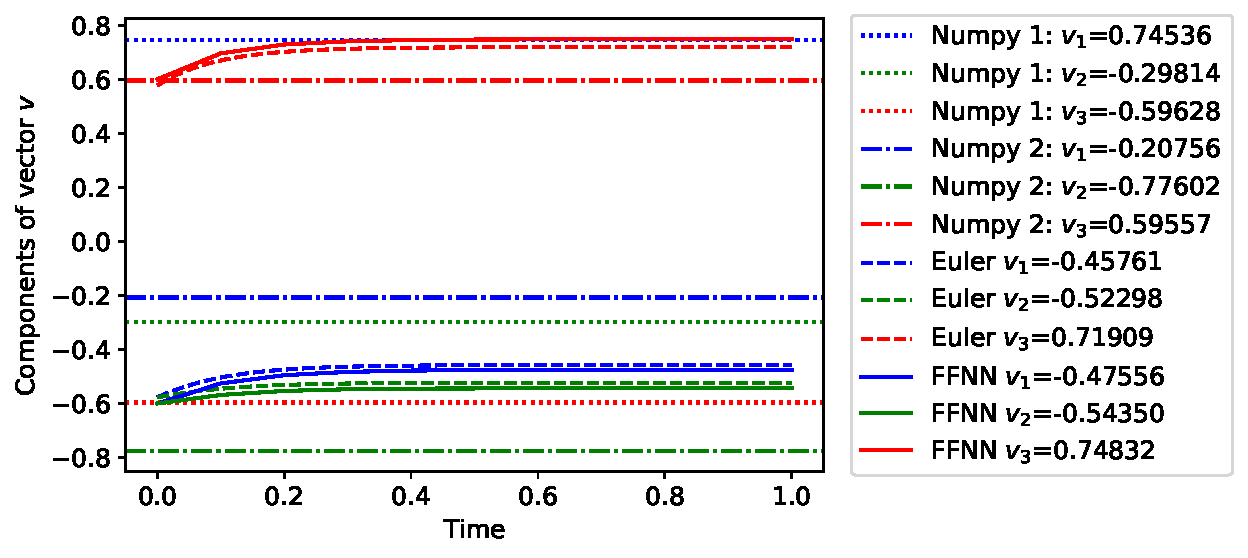
\includegraphics[scale=0.6]{latex/figures/eigvec_comp_benchrun3.pdf}}}
\qquad
\subfloat[]{{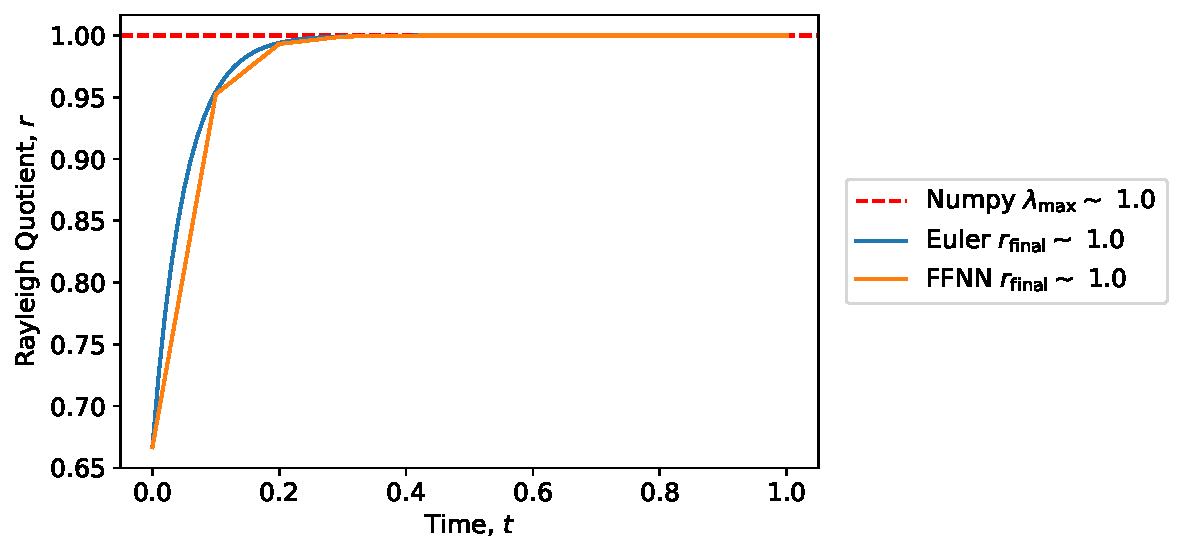
\includegraphics[scale=0.6]{latex/figures/eigval_benchrun3.pdf}}}
\caption{Results for Benchmark Problem 2 with a $3\times 3$ real symmetric matrix, $-A$. \textbf{(a)} shows the components of the computed steady-state vector as a function of time. The dashed lines are the components computed by Euler's method and the solid lines are computed by the FFNN model. In this case, there are two eigenvectors corresponding to the largest eigenvalue. The dotted and dotdashed lines are the normalized (unit "length") eigenvector components corresponding to the largest eigenvalue computed directly from the matrix by Numpy's linalg.eig. \textbf{(b)} shows the computed Rayleigh quotients, $r$, as a function of time for both Euler's method and the FFNN model and the largest eigenvalue, $\lambda_\mathrm{max}$, of the matrix computed by Numpy's linalg.eig as well. The final Rayleigh quotients are rounded to 5 decimal points.}
\label{fig:benchrun3}
\end{figure}

\begin{table}[H]
\caption{The computed Rayleigh quotients at the final simulation time for both Euler's method and the FFNN model. The absolute error relative to the eigenvalue computed by Numpy is also listed.}
\centering
\rowcolors{2}{gray!20}{white}
\begin{tabular}{c|c|c}
\hline
\hline 
Method & Rayleigh Quotient & Absolute Error
\\
\hline 
\hline 
Numpy & 1.0 & –
\\
Euler & 0.99999999 & $5.440 \cdot 10^{-10}$  
\\
FFNN & 0.99999626 & $3.736 \cdot 10^{-6}$
\\
\hline
\hline 
\end{tabular}
\label{tab:eigbench3}
\end{table}

DISCUSS

Shows that the computed steady-state vector not necessarily is the eigenvector if there are degenerated eigenvalues. However, the results indicate that the steady-state vector is a linear combination of the eigenvectors corresponding to the degenerated eigenvalues, which implies that the eigenvalue is the same nevertheless. 

Interestingly, the accuracy of the Rayleigh quotient compared to the actual eigenvalue improved 


%===============================================================
\subsubsection{Benchmark Problem 4}
%===============================================================

\autoref{tab:parabench4} tabulates the problem and model parameters for Benchmark Problem 4 described in \autoref{sec:benchmark problem 4}.

\begin{table}[H]
\caption{Problem and model parameters for Benchmark Problem 4.}
\centering
\rowcolors{2}{gray!20}{white}
\begin{tabular}{c|c}
\hline
\hline 
Parameter & Numerical Value
\\
\hline 
\hline 
Initial vector & $\bm{x_0}=(1, 0, -1)$
\\
Simulation time & 1
\\
Number of time points (Euler) & 101
\\
Number of time points (FFNN) & 11
\\
Number of epochs (FFNN) & 2000
\\
\hline
\hline 
\end{tabular}
\label{tab:parabench4}
\end{table}

\autoref{fig:benchrun4} shows the results for Benchmark Problem 3. The computed Rayleigh quotients and the absolute error relative to the eigenvalue computed by Numpy are tabulated in \autoref{tab:eigbench4}. 

\begin{figure}[H]
\begin{center}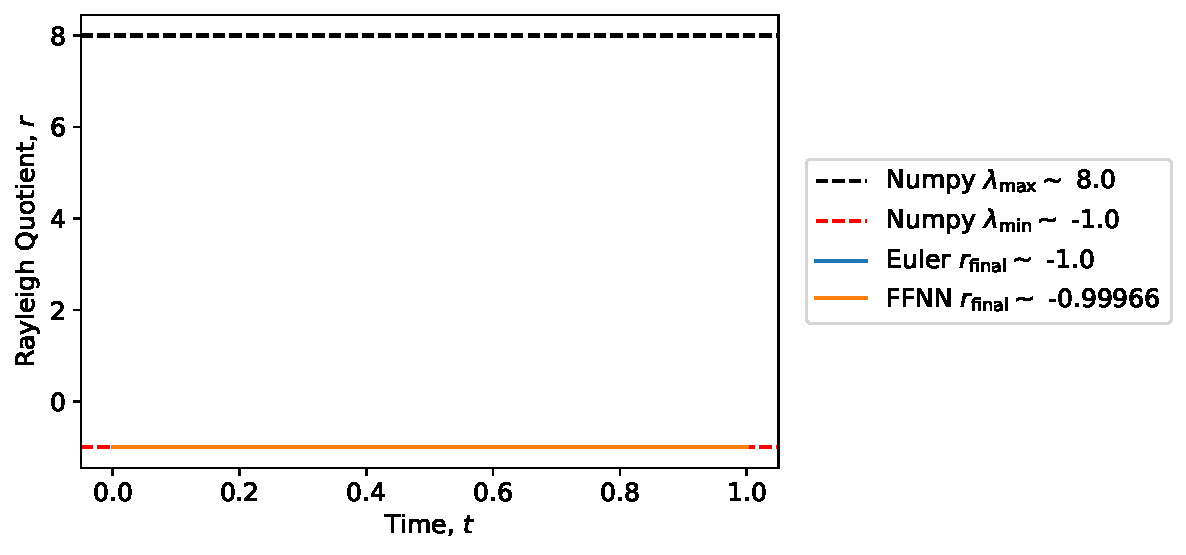
\includegraphics[scale=0.6]{latex/figures/eigval_benchrun4.pdf}
\end{center}
\caption{The computed Rayleigh quotients, $r$, as a function of time for both Euler's method and the FFNN model and the largest eigenvalue, $\lambda_\mathrm{max}$, of the matrix computed by Numpy's linalg.eig as well. The final Rayleigh quotients are rounded to 5 decimal points.}
\label{fig:benchrun4}
\end{figure}

\begin{table}[H]
\caption{The computed Rayleigh quotients at the final simulation time for both Euler's method and the FFNN model. The absolute error relative to the eigenvalue computed by Numpy is also listed.}
\centering
\rowcolors{2}{gray!20}{white}
\begin{tabular}{c|c|c}
\hline
\hline 
Method & Rayleigh Quotient & Absolute Error
\\
\hline 
\hline 
Numpy & 1.0 & –
\\
Euler & -0.99999999 & $1.110 \cdot 10^{-15}$  
\\
FFNN & -0.99965815 & $3.418 \cdot 10^{-4}$
\\
\hline
\hline 
\end{tabular}
\label{tab:eigbench4}
\end{table}

DISCUSS

Best Euler accuracy so far, FFNN not so much


%===============================================================
\subsubsection{Benchmark Problem 6}
%===============================================================

Benchmark Problem 5: 6x6 matrix and the effect of increased time and time points

T=10 
num epochs=2000
Number of time points for euler and ffnn stated in respective plot title

\autoref{fig:benchrun5}

\begin{figure}[H]
\centering
\subfloat[]{{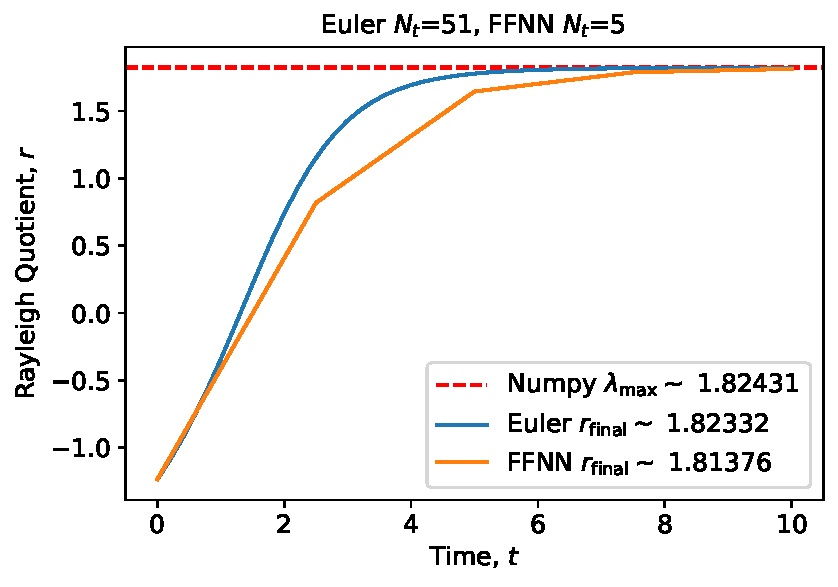
\includegraphics[scale=0.5]{latex/figures/eigval_run66a.pdf}}}
\qquad
\subfloat[]{{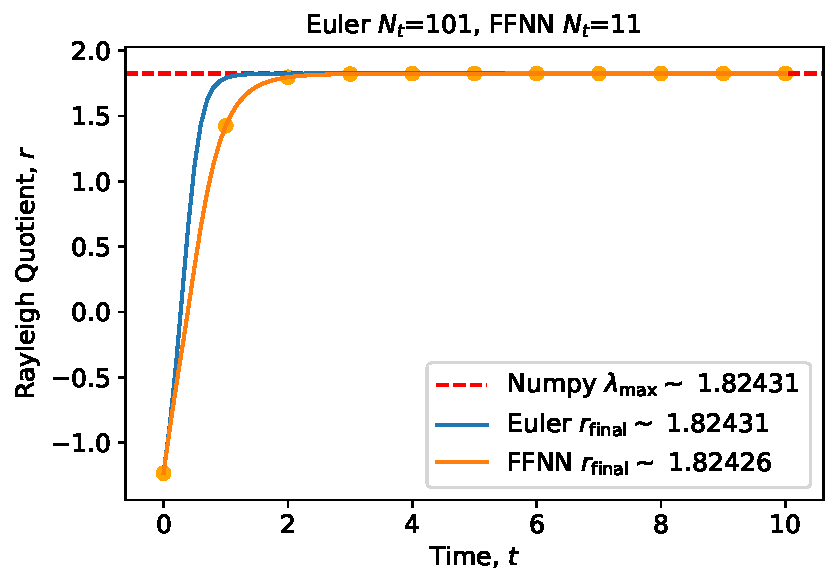
\includegraphics[scale=0.5]{latex/figures/eigval_run66b.pdf}}}
\qquad
\subfloat[]{{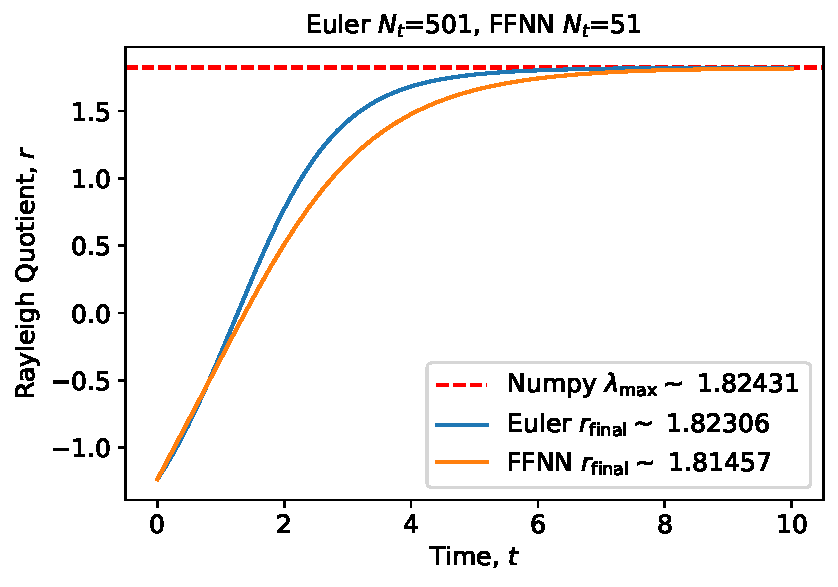
\includegraphics[scale=0.5]{latex/figures/eigval_run66c.pdf}}}
\qquad
\subfloat[]{{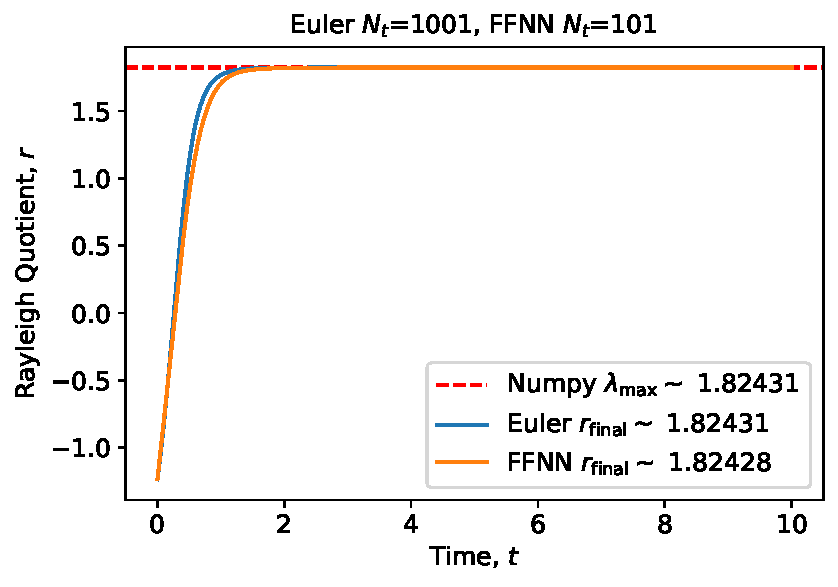
\includegraphics[scale=0.5]{latex/figures/eigval_run66d.pdf}}}
\caption{Results for Benchmark Problem 5 with a $6\times 6$ real symmetric matrix, $A$. The figure shows the time evolution of the Rayleigh quotient computed by Euler's method and the FFNN model with, respectively, the following time steps \textbf{(a)} 51 and 5, \textbf{(b)} 101 and 11, \textbf{(c)} 501 and 51, \textbf{(d)} 1001 and 101}
\label{fig:benchrun5}
\end{figure}

As seen in the above figure, the largest eigenvalue computed by Numpy is
\begin{equation*}
    \lambda_\mathrm{max} \approx 1.824312
\end{equation*}

The final Rayleigh quotients computed at different time steps and the absolute error relative to the eigenvalue computed by Numpy are tabulated in \autoref{tab:eigbench5}.

\begin{table}[H]
\caption{The computed Rayleigh quotients at the final simulation time for both Euler's method and the FFNN model with different time steps. The absolute error relative to the eigenvalue computed by Numpy is also listed.}
\centering
\rowcolors{2}{gray!20}{white}
\begin{tabular}{c|c|c|c}
\hline
\hline 
Method & Number of Time Steps & Rayleigh Quotient & Absolute Error
\\
\hline 
\hline 
Euler & 51 & 1.823322 & 0.000990
\\
Euler & 101 & 1.823180 & 0.001132
\\
Euler & 501 & 1.823055 & 0.001257
\\
Euler & 1001 & 1.823039 & 0.001273
\\
FFNN & 5 & 1.813760 & 0.010552
\\
FFNN & 11 & 1.816207 & 0.008105
\\
FFNN & 51 & 1.814569 & 0.009743
\\
FFNN & 101 & 1.814109 & 0.010202
\\
\hline
\hline 
\end{tabular}
\label{tab:eigbench5}
\end{table}

Results indicate small number of time steps for Euler and 1 point per unit time (sikkert en bedre måte å si det på) for FFNN is best. However, in the Euler case this may just be for this particular matrix. Other test runs with random matrices have shown a better convergence with a time step that is neither to small or to large. In the FFNN case, this result match those of the test runs. The accuracy of the FFNN can be improved by increasing the number of epochs at the cost of computational speed.  




